\chapter{Analysis}
In this chapter, we describe a method to automatic extraction landmarks from biological images. This method was proposed by Palaniswamy$^{\cite{palaniswamy2010automatic}}$ and the process includes some steps as follows:
\begin{enumerate}
\item Segmentation (includes preprocessing image and extracting the features),
\item Construction and comparison the Pairwise Geometric Histogram,
\item Estimation the global pose of object by the Probabilistic Hough Transform,
\item Refinement the estimated landmarks by template matching.
\end{enumerate}
\section{Segmentation}
Segmentation is a process to extract interested features (lines) from the digital image. The expected result in this process is the list of the approximate lines which are used to construct the pairwise geometric histogram. \\[0.2cm]
The process mainly separate into two stages: firstly, we pre-process image; secondly, we extract the image's features. In first stage, we reduce the noise in image by finding a threshold value and applying the thresholding technique to obtain the interested features. In second stage, we extract the features based on the edge segmentation. By applying the appropriate technique to obtain the step edges and broken the edges into approximate lines.
\subsection{Preprocess image}
In this application, we use the thresholding technique to pre-process the image. In thresholding technique, using a threshold value \textbf{``t"}, we can decrease the noise and obtain the interested features. The threshold value can be defined by the histogram analysis.\\[0.2cm]
Based on the histogram of the original image, we compute the mean and the median of this histogram. With the histogram obtained, we split it into two parts: the first part starts from the bin 0 to the limit value (the limit value is the smallest value between mean and median); the second part, starts from the limit value to the end of the histogram. For each part, we find the maximum, minimum value and calculating the mean of it. The value ``t" obtained by the mean of the two mean values in two parts of histogram.\\
With the threshold value ``t", we apply the threshold technique to pre-process image in the CV\_THRESH\_BINARY mode (keep the pixel has value greater than threshold value).\\
\IncMargin{1em}
\begin{algorithm}[H]
\Indm 
\KwData{inputImage: the input image}
\KwResult{outputImage: the image after processing}
\Indp
Convert the input image into gray scale image\;
Calculate the histogram on gray scale image and store the result in $histogram$ variable \;
Compute the $mean$ value and $median$ value of histogram\;
$limit \leftarrow (mean > median$ ? $median : mean)$\;
$limitSub \leftarrow ((limit >= 120)$ ? $(limit - 25) : (limit - 5))$\;
Declare some variables: $int$ $imax \leftarrow -1, max \leftarrow -1$\;
\For{$i \leftarrow$ 0 to $limitSub$}{
	\If{$histogram[i]$ $>$ $max$}{
		$max$ = $histogram[i]$\;
		$imax$ = $i$\;
	}
}
Declare some variables: $int$ $imin \leftarrow -1, min \leftarrow max$\;
\For{$k \leftarrow$ imax to $limit$}{
	\If{$histogram[k]$ $<$ $min$}{
		$min$ = $histogram[k]$\;
		$imin$ = $k$\;
	}
}
Declare some variables: $int$ $max2 \leftarrow -1, imax2 \leftarrow -1$\;
\For{$j \leftarrow limit $ to $end\_of\_histogram$}{
	\If{$histogram[j]$ $>$ $max2$}{
		$max2$ = $histogram[j]$\;
		$imax2$ = $j$\;
	} 
}
$middle1 \leftarrow (imax1 + imin)/2$ \;
$middle2 \leftarrow (imax2 + imin)/2$ \;
$middle \leftarrow (middle1 + middle2)/2$ \;
Apply the threshold with threshold value is $middle$\;
\caption{Algorithm to preprocess image}
\end{algorithm}\DecMargin{1em}
\subsection{Feature extraction}
After applying the threshold to pre-process image, we apply the Canny algorithm to detect the step edges, which incorporates non-maximal suppression and hysteresis thresholding. In Canny, the important parameters are the two threshold values and the aperture size of the Sobel operator, it decides the pixels kept. The threshold value used in Canny algorithm also the value used in the previous step, and the ratio between lower threshold and upper threshold is 1 : 3 (follows the article \cite{palaniswamy2010automatic} but have to be modified). In our implementation, the Canny operation used from OpenCV library\footnote{http://docs.opencv.org/modules/imgproc/doc/feature\_detection.html\#canny}, and the parameters need to be provided into Canny are:
\begin{itemize}
\item source: the input image (in grayscale mode)
\item destination: the output image,
\item low\_thresh: the first (lower) threshold value,
\item hight\_thresh: the second (upper) threshold value,
\item kernel\_size: size of kernel, aperture for the Sobel operator.
\end{itemize}
The Canny algorithm is not aware of the actual edges, the edge detecting process was based on the Sobel operator, extracted with non-maximal suppression. To obtain the expecting result, we apply another technique to obtain the step edges. The \textbf{findContours} was chosen for this goal, the result is a vector of the edges, and each edge was presented by a vector of the points. Like the Canny, the \textbf{findContours} uses OpenCV library \footnote{http://docs.opencv.org/modules/imgproc/doc/structural\_analysis\_and\_shape\_descriptors.html\#findcontours} and the parameters used in this operation are as follows:
\begin{itemize}
\item source: the binary input image,
\item contours: the output. Each contours is stored in a vector of points,
\item hierarchy: optional output vector, containing information about the image topology,
\item mode: contours retrieve mode,
\item method: contours approximation method,
\item offset: optional offset by which every contour point is shifted.
\end{itemize}
\subsection{Edge segmentation}
The geometric relation could not be constructed from the edges, it is always constructed from the relation of basic geometric objects, such as the lines.  In fact, any arbitrary edge can be represented by a set approximate lines. Instead an edge, we represent a set of approximate lines of it. This method is useful when we want to present the edges or describe the relationship between the lines. From the set of step edges was obtained from find contours (the image structure), in this step, we will segment each step edge into approximated lines. The method to segment the edges is the recursive algorithm$^{\cite{thacker1995assessing}}$ but it has some changes in the ``stop condition" of the algorithm to simplify, as follows:
\begin{itemize}
\item Establish a line \textit{``l"} between two endpoints of the edge.
\item For each point on edge, we compute the perpendicular distance from it to the line l and keep the point which has the maximum perpendicular distance.
\item If the maximum perpendicular distance from a point on edge to the line \textit{l} is greater than $\alpha$, then the edge is splited at this point. The value chosen for $\alpha$ in the program is 3 ($\alpha = 3$).
\item Reprocess both parts which was obtained from step 3.
\item The algorithm continues until all edges fragments are represented.
\end{itemize}
The algorithm is presented as follows:\\
\IncMargin{1em}
\begin{algorithm}[H]
\Indm 
\KwData{listPoints: list of points which presented the edge}
\KwResult{Queue of ``step" points on the edge}
\Indp
Declare the first endpoint: $p0 \leftarrow listPoints[0]$\;
Declare the second endpoint: $pend \leftarrow listPoints[size - 1]$, \textit{size} is the size of \textit{listPoints}\;
Set up a straight line between the two endpoints $p0, pend$ (line $d$)\;
Initialization the max value: $maxDistance  \leftarrow 0 $\;
Declare a ``split point": $imax \leftarrow 0$ \; 
Declare a variable: $distance \leftarrow 0$\;

\For{ point $p$ in $listPoints$}{
	$distance \leftarrow$ from $p$ to line $d$\;
	\If{distance $>$ max\_distance}{
		$maxDistance$ $\leftarrow$ $distance$\;
		$imax$ $\leftarrow$ position of $p$\;
	}
}
\If{$maxDistance$ $>$ 3 }{
	split the list of points at $imax$ and put into 2 parts $(part1, part2)$\;
	Pre-process on $part1$\;	
	Pre-process on $part2$\;
}
\If {$p0$ does not exist in result queue}{
	push $p0$ into queue\;\tcp{queue is a variable of class}
}
\If {$pend$ does not exist in result queue}{
	push $pend$ into queue\;\tcp{queue is a variable of class}
}
\caption{Algorithm to segment an edge}
\end{algorithm}\DecMargin{1em}
\section{Pairwise Geometric Histogram}
Pairwise Geometric Histogram(PGH)$^{\cite{evans1993use}}$ is used to encode the relative information between a line and a set of lines in an object. Therefore, an object can be represented by a set of PGH. From the set of PGH, we can reconstructed the object or compare to another object. In this section, we introduce the construction of a PGH for an object based on the geometrical relationship and compute the similar distance between two objects.

\subsection{Local pairwise geometric histogram}
The PGH is constructed on the geometric features between lines relative. The geometric features are characteristic which can describe the geometric shape such as angle, the length of line, perpendicular between two lines, .... For the shape representation, the relative angle and perpendicular distance is geometrical features useful. \\
The proceed to construct the PGH between two lines was described in below:
\begin{itemize}
\item Choose the reference line (other lines called object lines),
\item Compute the angle between the reference line and the object lines,
\item Calculate the perpendicular distance from the two endpoints of an object lines to the reference line (assigned dmin and dmax),
\item Recording the perpendicular distance and the angle relation between reference line and the object lines into the two-dimensional histogram.
\end{itemize}
\begin{figure}[h!]
\centering
\subfloat[The geometric relationship between two lines]{\label{fig:example_1}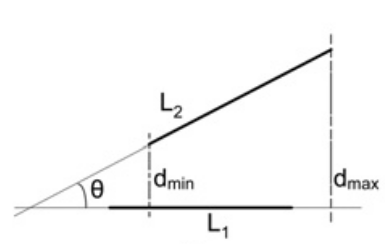
\includegraphics[width=0.3\textwidth]{./images/PGH_geo}}~~
\subfloat[The pairwise geometric histogram ]{\label{fig:example_2}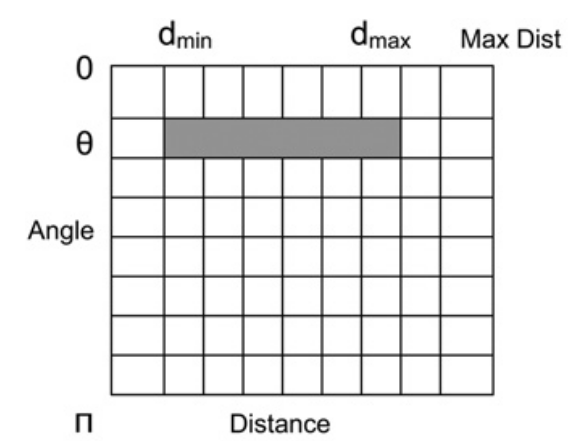
\includegraphics[width=0.3\textwidth]{./images/PGH}}
\caption{Example about geometric features and the pairwise geometric histogram}
\label{fig:figure_31}
\end{figure}
The local PGH presented the relationship between a reference line with other lines of shape. Thus, for an object, we can construct a local PGH for each line in object. The frequency of the geometric features is recorded as a two dimensional histogram with an angle axis (0 - $\pi$) and distance axis (range of perpendicular distance, $d_{max}$ is the maximum distance on all distance of two arbitrary lines). The entries on PGH describes the geometric relationship between the reference line and the object lines. The blurring of entry along the axis regarding the true position and orientation of each object lines for reference line. Following the accuracy, we can indicate the size of histogram and normalize the value to match with size of histogram.
\subsection{Global pairwise histogram}
Based on local PGH constructor, global pairwise histogram is combined of all local PGHs of all lines belong to the object. It means if the object is defined by n lines, the global pairwise histogram will composed of n local PGHs. This method is good when we apply some variants on the image, such as translate or rotate the image because the angle and perpendicular distance between a pair of lines are invariant.
\subsection{Histogram matching}
\textbf{``The histogram matching enables robust classification of shape features by finding similarity between the scene and reference model"}$^{\cite{palaniswamy2010automatic}}$. The similar between two models can obtain via the similar distance, which is computed by comparing their probability distribution on geometric histogram. In our program, each image is represented by a comprises of many geometric histograms and uses the Bhattacharya metric to determine the similar distance between the two models $^{\cite{palaniswamy2010automatic}}$. In general, we have normalize the histograms before comparing. The form of Bhattacharrya metric used to compute the degree of 2 model:
\begin{center}
\begin{equation} \label{eq:1}
d_{Bhattacharyya} (H_{i}H_{j}) = \sum\limits_{\theta}^{\pi}\sum\limits_{d}^{d_{max}}\sqrt{H_{i}(\theta,d)H_{j}(\theta,d)}
\end{equation}
\end{center}
The significance of parameters in the formula \ref{eq:1}, as follows:
\begin{itemize}
\item $\theta$: angle value, range of $\theta$ in angle axis from 0 to $\pi$.
\item $d$: the perpendicular distance, range of d in perpendicular distance from 0 to the maximum distance of arbitrary lines of shape.
\item $H_{i}(\theta,d)$ is an entry at row $\theta$ and column d in histogram of image \textit{i}
\item $H_{j}(\theta,d)$ is an entry at row $\theta$ and column d in histogram of image \textit{j}
\end{itemize}
Based on the accuracy of the program, we can change the range of the angle and distance axis. 
Besides the Bhattacharya metric, we may choose another metric to matching the histograms, such as: \textbf{Chi-squared} metric and \textbf{Intersection} metric. The forms are presented as below:\\
\textbf{Chi-squared metric:}
\begin{center}
\begin{equation}\label{eq:2}
d_{Chi-squared} (H_{i}H_{j}) = \frac{\sum\limits_{\theta}^{\pi}\sum\limits_{d}^{d_{max}}(\frac{(H_{i}(\theta,d) - H_{j}(\theta,d))^{2}}{(H_{i}(\theta,d) + H_{j}(\theta,d))})}{2}
\end{equation}
\end{center}
\textbf{Intersection metric}
\begin{center}
\begin{equation}\label{eq:3}
d_{Intersection} (H_{i}H_{j}) = \sum\limits_{\theta}^{\pi}\sum\limits_{d}^{d_{max}}min(H_{i}(\theta,d), H_{j}(\theta,d))
\end{equation}
\end{center}
The significance of parameters in formula (\ref{eq:2}) and (\ref{eq:3}) are similar to formula (\ref{eq:1}). For the Bhattacharyya and Intersection metric, the perfect match is 1 and the total mismatch is 0. The result is opposite to Chi-squared metric (0 for perfect match and 1 for total mismatch).\\[0.2cm]
Hence, depending on the purpose of the comparison subject will choose a suitable comparing method. In this program, we propose three methods to obtain a general result when matching the histograms.
\section{Probabilistic Hough transform}
The Probabilistic Hough Transform (PHT) is used to estimate the global pose of shape$^{\cite{ashbrook1995robust}}$. Based on a group of features within the scene, identifying the represent of a model image in a scene image. The hypothesised location of the model in the scene is indicated based on the conditional probability that any pair scene lines agreement about a position in model.\\[0.3cm]
Estimating the global shape has two main stages. Firstly, training process starts with recording the perpendicular distance and the angle from a reference point to each pair of model lines. Secondly, predicting the pose of scene different from the model, then we estimate the location of the landmarks. We create a Hough space to store value if exist a pair of scene lines matching to the entry in the training process. The peak in Hough space is assumed as the reference point of the model in the scene image. From this reference point, we can estimate the reference landmarks of reference image on the scene image.
The process to estimate the global pose includes the steps as follows:
\begin{itemize}
\item Choose an arbitrary point in the model as a reference point,
\item For each pair lines in the model, calculating and recording the perpendicular distance and angle from the reference point to each line,
\item Create an two-dimensional accumulator, one dimension for the angle and the other for the perpendicular distance,
\item For each pair lines in the scene, finding the entry correspond to the position, orientation and scale. Increasing the value at correlative cell in the accumulator (indicate by the angle and distance),
\item Compute the maximum value in the accumulator,
\item Indicating the pair of scene lines and the entry with maximal value of accumulator,
\item Extending the perpendicular lines of the pair belong to scene lines at the appropriate position. The intersection of them is the location of the reference point in the scene.
\end{itemize}
In the example below, we apply the PHT to estimate the landmarks of the model to the scene. The image in figure \ref{fig:pht_1} as the model. In the model, the small red circle and large red circles are the reference point and the landmarks in model, respectively. The image in figure \ref{fig:pht_2} as scene. By applying the PHT, we estimate the reference point (green circle) in the scene and the location of the landmarks (the yellow circles).
\begin{figure}[h!]
\centering
\subfloat[The model image]{\label{fig:pht_1}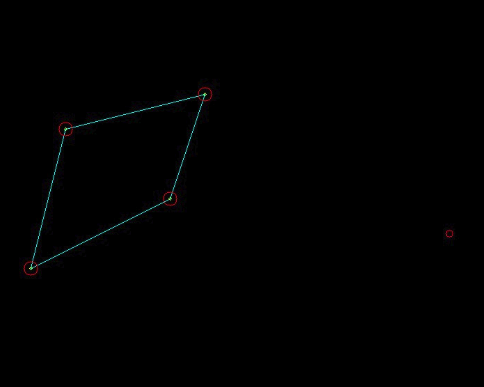
\includegraphics[width=0.45\textwidth]{./images/pht_1}}~~
\subfloat[The scene image ]{\label{fig:pht_2}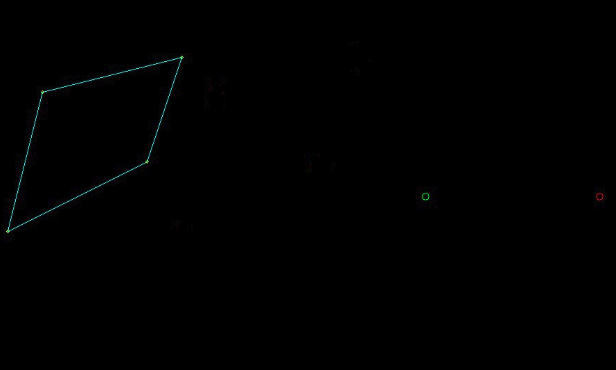
\includegraphics[width=0.45\textwidth]{./images/pht_2}}
\caption{The landmarks estimated by probabilistic Hough transform}
\label{fig:figure_31}
\end{figure}
\subsection{Training process}
In this step, recording the perpendicular distance and angle from each pair model lines to a reference point (called reference table). The reference point can be chosen at arbitrary position on the model image. To reduce the time complexity processing the next step, we consider the ``closet pair lines". In this application, the reference point chosen at the center of image and the closet pair lines are pair of lines have all three conditions: the length of each line greater than 60 pixels, the lines are not parallel and the distance between them is less than 5 pixels. The algorithm considers a pair of closet lines and constructs the reference table as follows:\\[0.2cm]
\begin{algorithm}[H]
\Indm 
\KwData{line1 (the first line), line2 (the second line)}
\KwResult{Two line closet or not (bool)}
\Indp
$distance1$ $\leftarrow$ distance from the first endpoint of $line1$ to $line2$\;
$distance2$ $\leftarrow$  distance from the second endpoint of $line1$ to $line2$\;
\If {$line1.length() > $ 60 and $line2.length() > $60  \\
		and $line1$ not parallel with $line2$\\
		and ($distance1$ $<=$ 5 or $ditance2$ $<=$ 5 )}{
	$return$ $true$\;
}
return $false$\;
\caption{Algorithm to consider the closet lines}
\end{algorithm}~\\[0.2cm]
\begin{algorithm}[H]
\Indm 
\KwData{lines (a list of lines), refPoint (the reference point)}
\KwResult{The reference table}
\Indp
Declare the reference table $refTable$ \;
\For{ line $i$ in $lines.size()$}{
	\For{line $j$ in $lines.size()$}{
		\If{i $!=$ j and $line(i)$ closet with $line(j)$}{
			Compute the angle and perpendicular distance from $line(i)$ to $refPoint$\;
			Compute the angle and perpendicular distance from $line(j)$ to $refPoint$\;
			Create an entry to store pair of lines and its information \;
			Add the entry into reference table \;
		}
	}
}
return $refTable$ \;
\caption{Algorithm to construct the reference table}
\end{algorithm}~\\
\subsection{Estimating process}
The estimating process is duration that estimating the reference landmarks on the scene image. Firstly, we find the reference point on scene image. Secondly, we estimate the reference landmarks on the scene image from the position of reference point in the scene image.\\[0.2cm]
By finding a pair of scene lines agree with a pair of model lines, we can detect the position of the reference point on scene image. We create an accumulator to store each agreement between the pair of scene lines and the pair of model lines. For each pair of scene lines, we find its exist in the reference table and increase the value at correspondence position in accumulator. At the end, we obtain a pair of scene lines and pair of model lines correspondence with the maximum value in accumulator. By extending the perpendicular lines of the pair of scene lines at the appropriate position, we meet the reference point at the intersection.\\[0.2cm]
In our program, two pair lines are supposed to be agreement if the angle difference between them is less than one degree, the length scale is less than 1 and the distance between two pair of lines is less than two. Two followed algorithms describe the definition between the two pair lines and finding the position of reference point in scene image.\\[0.2cm]
\begin{algorithm}[H]
\Indm 
\KwData{line1 (the first reference line), line2 (the second reference line), sline1 (the first scene line), sline2 (the second scene line)}
\KwResult{Two pair lines similar or not (boo)}
\Indp
$angle1$ $\leftarrow$ angle between $line1$ and $line2$\;
$angle2$ $\leftarrow$ angle between $sline1$ and $sline2$\;
$mdistance$ $\leftarrow$ sum of perpendicular distance from two endpoints of $line1$ to $line2$\;
$sdistance$ $\leftarrow$ sum of perpendicular distance from two endpoints of $sline1$ to $sline2$\;
\If{$abs(ange1$ - $angle2) < 1$ \\
	$and$ $abs(line1.length()/sline1.length()$ - $line2.length()/sline2.length()) < 1$ \\
	$and$ $abs(mdistance$ - $sdistance) < 2$}{
	return $true$\;
}
return $false$ \;
\caption{Algorithm to check the agreement between two pair lines}
\end{algorithm}~\\[0.2cm]
\begin{algorithm}[H]
\Indm 
\KwData{refTable (the reference table), slines (pair of scene lines)}
\KwResult{The entries in reference table similar with pair of scene lines}
\Indp
Declare the return entries in reference table $entries$ \;
\For{ entry $et$ in $refTable$}{
	\If{agree between lines in entry and $slines$}{
		put the entry $et$ into list of entries $entries$\;
	}
}
return $entries$ \;
\caption{Algorithm to find the agreement of pair scene lines in model}
\end{algorithm}~\\[0.2cm]
\begin{algorithm}[H]
\Indm 
\KwData{lines (a list of scene lines), refTable (reference table)}
\KwResult{The reference table}
\Indp
Create an accumulator, $acc$\;
Declare the reference table $refTable$ \;
\For{ line $i$ in $lines.size()$}{
	\For{line $j$ in $lines.size()$}{
		\If{i $!=$ j and $line(i)$ closet with $line(j)$}{
			Find the agreement of pair scene lines in mode\;
			Increase the value in $acc$ with correspondence position\;
			Marked the maximum value, pair of scene lines and entry in reference table\;
		}
	}
}

Find the intersection ($intersect$) between two perpendicular lines with pair scene lines at appropriate position\;
\tcp{The appropriate position is correct with the distances in reference table.}
return $intersect$ \;
\caption{Algorithm to find the reference point in scene}
\end{algorithm}~\\[0.2cm]
By finding the reference point, the landmarks in the scene image can be estimated by calculating the relatedness between the reference point and the reference landmarks. Besides, we also record the difference about rotation, orientation and scale between the model image and the scene image.
\section{Template matching}
Template matching is the process to refine the estimated landmarks, which was obtained by PHT of the scene image with an appropriate method.
\subsection{Cross-correlation}
Cross-correlation is a method of estimating the similarity between the two signals. By computing the sum of products between two signals when sliding, and choose the maximal value. It is used for searching a short signal in a longer signal. In image processing, it used to detect the present of an object (template) in a large object (image). The equation of cross-correlation is as follows (equation \ref{eq:cross-correlation}):
\begin{center}
\begin{equation}\label{eq:cross-correlation}
R_{ccorr}(x,y) = \sum\limits_{x',y'}[T(x'.y').I(x + x', y + y')]
\end{equation}
\end{center}
Where:
\begin{itemize}
\item T is template which use to slide and find the exist in other image.
\item I is image which we expect to find the template image
\item $(x', y')$ are coordinates in template where we get the value to compute.
\item $(x + x', y + y')$ are coordinates in image where we get the value to compute when template $T$ sliding.
\end{itemize}
By sliding the template on image by each pixel from left to right and top to down. At each position, we compute the $R_{ccorr}(x,y)$. The position have maximal $R_{ccorr}(x,y)$ is positioned that best similar of template in image.\\[0.2cm]
However, if we use the original image to compute and find the similarity, the brightness of the template and the image might change the conditions and the result. So, we can normalize the image before applying the cross-correlation to reduce the effect of lighting difference between them. The normalization coefficient is:
\begin{center}
\begin{equation}\label{eq:normalizeCoff}
Z(x,y) = \sqrt{\sum\limits_{x',y'}T(x'.y')^{2}.\sum\limits_{x',y'}I(x + x', y + y')^{2}}
\end{equation}
\end{center}
The value of this method when we normalized computation as below:
\begin{center}
\begin{equation}\label{eq:cross-correlation}
R_{ccorr\_norm}(x,y) =\frac{R_{ccorr}(x,y)}{Z(x,y)} = \frac{\sum\limits_{x',y'}[T(x'.y').I(x + x', y + y')]}{\sqrt{\sum\limits_{x',y'}T(x'.y')^{2}.\sum\limits_{x',y'}I(x + x', y + y')^{2}}}
\end{equation}
\end{center}
\subsection{Template matching}
Back to our problem, with a reference image and its set of landmarks. We use the cross-correlation to refine the landmarks. In this case, the template is a region around each landmark in reference image and the image is also a region around the Hough landmark detection in scene image. Hence, to save the processing time, before applying the cross-correlation, the scene image is rotated to match with model using Hough estimate.\\[0.2cm]
For each landmark in the reference image, we create a bounding box around the landmarks with an arbitrary size and use landmark as a center point. When create the bounding box, we need to keep the distance between left corner to the landmarks, because sometimes, with the landmark position, the size of bounding box can be over the size of image. Use this box as a template and do the cross-correlation with each scene image. The results obtained store the location where the template matches the image. From these position, we indicate the position of each landmark of reference image on scene image. The algorithm to create the bounding box around a landmark is described follows:\\[0.2cm]
\begin{algorithm}[H]
\Indm 
\KwData{image (reference image), landmark (location of a reference landmark), tsize (size of bounding box), distance (to keep the distance from the landmark to bounding box)}
\KwResult{A matrix represented for bounding box of landmark}
\Indp
Get the matrix of image (image presented by matrix): $Mat matImg = image.getMatrix()$\;
\tcp{Indicate the top left-corner of bounding box:}
$int$ $lx = (landmark.x - tsize/2) < 0$ ? $0$ : $(landmark.x - tsize/2)$\;
$int$ $yx = (landmark.y - tsize/2) < 0$ ? $0$ : $(landmark.y - tsize/2)$\;
\tcp{Keep the distance from the landmark to bounding box}
$distance.x = landmark.x - lx$\;
$distance.y = landmark.y - ly$\;
\tcp{Indicate the low right-corner of bounding box}
$int$ $lx2 = (landmark.x + tsize/2) > matImg.cols$ ? $matImg.cols$ : $(landmark.x + tsize/2)$\;
$int$ $yx2 = (landmark.y + tsize/2) < matImg.rows$ ? $matImg.rows$ : $(landmark.y + tsize/2)$\;
\tcp{Create the bounding box around landmark}
$Mat$ $box(matImg,Rect(lx,ly,lx2 - lx, ly2 - ly))$\;
return the $box$;
\caption{Algorithm to create a bounding box around a landmark}
\end{algorithm}~\\[0.2cm]
The belows algorithm describe a method to estimate the reference landmarks on a scene image by using cross-correlation. Before applying the cross-correlation, the scene image is rotated to match with the model. The angle used to rotate is the sum of the difference between the scene line and model line to which it matched and the difference between the two pairs of the similar lines. To apply the cross correlation, we have used the function $matchTemplate$\footnote{http://docs.opencv.org/modules/imgproc/doc/object\_detection.html?highlight=matchtemplate\#matchtemplate} in OpenCV library with matching method is $CV\_CCORR\_NORMED$ (cross-correlation normalize). This function allows us compare the template overlaping the image and it supports many different matching methods. When the template slide over each pixel on image, the coefficient between them is calculated and stored in a array.\\[0.2cm]
After finished correlation, to get the value and the position of the maximum value when we compute the coefficient, we use a function in OpenCV,  $minMaxLoc$\footnote{http://docs.opencv.org/modules/core/doc/operations\_on\_arrays.html?highlight=minmaxloc\#minmaxloc}. This method is used to detect the minimum and maximum value in an array. Beside that, it also output the location where having the minimum and maximum value.\\[0.2cm]
\begin{algorithm}[H]
\Indm 
\KwData{refImage (reference image), sceneImage (the scene image), lmpath (file path store the reference landmarks)}
\KwResult{A list of landmarks on scene image}
\Indp
Get the reference landmarks from file and store in list $refLandmarks$\;
Create a variable to store the new landmarks: $sceneLandmarks$\;
Estimate the reference landmarks ($refLandmarks$) in scene image using probabilistic Hough transform and save into a variable: $esLandmarks$\;
\tcp{Get the matrix of scene image}
$sceneMatrix$ = $sceneImage.getMatrix()$\;
Rotate the scene matrix with appropriate angle\;
\For{ variable $i$ in $esLandmarks.size()$}{
	\tcp{Get the reference landmark}
	$Point$ $refPoint$ = $refLandmarks.at(i)$\;
	\tcp{Create a bounding box of reference landmark $refPoint$} 
	$Mat$ $template$ = $createTemplate(refImage, refPoint, size )$\;
	\tcp{Get the estimate landmark}
	$Point$ $esPoint$ = $esLandmarks.at(i)$\;
	\tcp{Create a bounding box of estimate landmark $esPoint$} 
	$Mat$ $sceneImg$ = $createTemplate(sceneImage, esPoint, size )$\;
	Create the matrix to store the value when do the cross-correlation: $result$ \;
	\tcp{Apply the matching and store the result into matrix $result$}
	$cv::matchTemplate(sceneMatrix,template,result,CV\_TM\_CCORR\_NORMED$\;	
	\tcp{Get the maximum value and position in $result$ matrix}
	$double$ $maxValue, minValue$\;
	$Point$ $maxLoc, minLoc$\;
	$cv::minMaxLoc(result, \&minValue, \&maxValue, \&minLoc, \&maxLoc, Mat())$\;
	Compute the position of landmark from maximum position\;
	Push the landmark into the list $sceneLandmarks$\;
}
Return the list of landmarks\;
\caption{Algorithm to get the position of reference landmarks in scene image}
\label{alccross}
\end{algorithm}~\\[0.2cm]
